\documentclass[11pt]{article}

\usepackage[a4paper,margin=1in]{geometry}
\usepackage[T1]{fontenc}
\usepackage[utf8]{inputenc}
\usepackage{lmodern}
\usepackage{microtype}
\usepackage{amsmath,amssymb,amsthm,mathtools}
\usepackage{booktabs}
\usepackage{array}
\usepackage{graphicx}
\usepackage{float}
\usepackage{placeins}
\usepackage{enumitem}
\usepackage[numbers,sort&compress]{natbib}
\usepackage{xcolor}
\usepackage{xurl}
\usepackage[colorlinks=true,linkcolor=blue!55!black,citecolor=blue!55!black,urlcolor=blue!55!black]{hyperref}
\usepackage[nameinlink,noabbrev]{cleveref}

\setlength{\parindent}{1.4em}
\setlength{\parskip}{0.15em}
\setlist{itemsep=0.25em,topsep=0.35em}
\allowdisplaybreaks

\newtheorem{theorem}{Theorem}[section]
\newtheorem{proposition}[theorem]{Proposition}
\newtheorem{lemma}[theorem]{Lemma}
\newtheorem{corollary}[theorem]{Corollary}
\theoremstyle{definition}
\newtheorem{definition}[theorem]{Definition}
\theoremstyle{remark}
\newtheorem{remark}[theorem]{Remark}

\newcommand{\C}{\mathbb C}
\newcommand{\Id}{\mathrm I}
\newcommand{\norm}[1]{\left\lVert#1\right\rVert}
\newcommand{\Atilde}{\widetilde A}
\newcommand{\Gmat}{\mathcal G}
\newcommand{\Tmat}{\mathcal T}
\newcommand{\Bhat}{\widehat B}
\newcommand{\up}{\operatorname{up}}
\newcommand{\inn}{\operatorname{In}}

\hypersetup{
  pdftitle={Two-Shift Sparse Inertia Certification of Lifted Grushin Resolvents},
  pdfauthor={Liang Wang},
  pdfsubject={Exact-target sparse threshold-inertia certificates at three stored finite scales},
  pdfkeywords={verified inertia, singular value, sparse LU, Grushin problem, Weyl monotonicity, interval arithmetic}
}

\title{\textbf{Two-Shift Sparse Inertia Certification of\\
Lifted Grushin Resolvents}\\[0.35em]
\large Exact-Target Weyl Certificates at Three\\
Quadratic Band-Merging Scales}
\author{Liang Wang\\
\small School of Artificial Intelligence and Automation,\\[-0.2em]
\small Huazhong University of Science and Technology, Wuhan 430074, P.R. China\\
\small \texttt{wangliang.f@gmail.com}}
\date{July 2026}

\begin{document}
\maketitle

\begin{abstract}
A preceding sparse Grushin linearization reduced a lifted nonnormal
resolvent gate to the inverse norm of one bordered matrix, but its rigorous
certificate constructed every physical inverse column.  This paper replaces
that all-column calculation by a fixed number of sparse factorizations.

For a square Grushin matrix $\Gmat\in\C^{m\times m}$ and threshold
$\alpha>0$, consider the Hermitian singular-value dilation
\[
 H_\alpha=
 \begin{pmatrix}
  -\alpha\Id&\Gmat\\
  \Gmat^*&-\alpha\Id
 \end{pmatrix}.
\]
Its inertia is $(m,m,0)$ exactly when
$s_{\min}(\Gmat)>\alpha$.  An unnormalized pairwise Hadamard congruence
turns this matrix into
\[
 \Tmat_\alpha=
 \begin{pmatrix}
  \Gmat+\Gmat^*-2\alpha\Id&\Gmat^*-\Gmat\\
  \Gmat-\Gmat^*&-\Gmat-\Gmat^*-2\alpha\Id
 \end{pmatrix},
\]
using only integer coefficients.  For independently chosen
$\delta_-,\delta_+>0$, sparse no-pivot LU factorizations of
$\Tmat_\alpha-\delta_-\Id$ and
$\Tmat_\alpha+\delta_+\Id$ are converted to exact Hermitian matrices
$\Bhat_\pm=L_\pm\operatorname{Re}(\operatorname{diag}U_\pm)L_\pm^*$.
If their normwise backward errors satisfy
$\varepsilon_-<\delta_-$ and $\varepsilon_+<\delta_+$ and their inertias
agree, Weyl monotonicity sandwiches the exact inertia of
$\Tmat_\alpha$ between them.  The two shift distances need not agree.

The target is not a rounded surrogate.  Peripheral, packet, and normalized
rank-one lift channels are enclosed componentwise from the exact archived
binary64 factors; channel balancing uses exactly reversible powers of two.
The resulting Grushin enclosure, threshold-transform rounding, shifted
assembly, complex sparse-LU backward error, and $LU$-to-$LDL^*$ conversion
are all included in one Frobenius majorant.  No inverse norm of $L$ and no
inverse columns are required.

At $\sigma=10^{-2}$, $4\times10^{-3}$, and $2\times10^{-3}$, the exact
target certificates have Grushin dimensions $4109$, $10255$, and $20497$.
The largest threshold matrix has dimension $40994$, $5.424\times10^7$
nonzeros, and $2.979\times10^8$ factor nonzeros per side.  Its two verified
errors are $1.43035\times10^{-3}$ and $1.43152\times10^{-3}$, both below
$1.5\times10^{-3}$, with common inertia $(20497,20497,0)$.  At every scale
we choose $\alpha>2/K_*^-$, where $K_*^-$ is the preceding rigorous lifted
inverse budget.  Hence
$\|\Atilde^{-1}\|_2\leq\|\Gmat^{-1}\|_2<K_*^-/2$, closing the three selected
stored-model lifted gates.

The result is finite-dimensional and local to three archived scales.  It
does not prove a full-contour root count, a continuum limit, a
Hilbert--P\'olya construction, an identification with zeta zeros, or the
Riemann hypothesis.
\end{abstract}

\noindent\textbf{Keywords:} verified inertia; sparse LU; singular-value
dilation; Grushin problem; nonnormal resolvent; interval arithmetic;
Weyl monotonicity.

\medskip
\noindent\textbf{MSC 2020:} 15A18; 15A23; 47A10; 65F05; 65F15; 65F50;
65G20; 65P30.


\section{Introduction}
\label{sec:introduction}

The finite packet--complement program considered here studies stored noisy
transfer matrices near a quadratic band-merging regime.  Earlier layers
constructed a contour Feshbach reduction, directional and primal--dual
residual identities, componentwise outward enclosures, and an adaptive
arcwise cover.  A one-channel deflation then isolated a single dangerous
singular direction and reduced the remaining analytic gate to a rigorous
upper bound for a lifted complement inverse
\citep{WangDeflated2026}.  The immediate predecessor supplied an exact
sparse two-step Grushin linearization and closed that gate at two scales by
constructing all physical inverse columns and checking a direct
Frobenius--Neumann residual \citep{WangSparseGrushin2026}.

That method was sharp but structurally expensive.  If the physical dimension
is $n$, it solves for $n$ right-hand sides and re-evaluates the exact target
on every resulting column.  The present paper asks a narrower question:
can one certify only the threshold inequality actually needed by the
preceding theorem,
\begin{equation}
 s_{\min}(\Gmat)>\alpha,
 \label{eq:intro-threshold}
\end{equation}
using a fixed number of sparse factorizations?

The answer is yes at the first three archived scales.  The route has four
parts.
\begin{enumerate}
 \item A Hermitian dilation turns \cref{eq:intro-threshold} into an inertia
       statement.
 \item An exact unnormalized Hadamard congruence stabilizes the paired
       diagonal structure without introducing irrational coefficients.
 \item Each no-pivot sparse LU factorization is converted to an exact
       Hermitian $LDL^*$ center whose inertia is read from real pivot signs.
 \item Two independently shifted centers sandwich the exact target by
       Weyl monotonicity.
\end{enumerate}
The key refinement is that the lower and upper shifts need not be symmetric.
This matters numerically: at the middle scale, one symmetric choice makes
the upper factorization unstable, while a nearby symmetric choice makes the
lower factorization unstable.  Selecting the stable side of each pair gives
a rigorous asymmetric bracket.

The contributions are:
\begin{enumerate}
 \item an exact threshold-inertia equivalence and integer pair congruence;
 \item an asymmetric two-shift Weyl sandwich theorem;
 \item a normwise sparse complex-LU and $LDL^*$ conversion certificate using
       only $O(\operatorname{nnz}(L)+\operatorname{nnz}(U))$ postprocessing;
 \item a componentwise enclosure connecting the factorized center to the
       exact RH-29 lifted target, including exact vector normalization;
 \item rigorous certificates at three scales, including the first closure
       at $\sigma=2\times10^{-3}$;
 \item a transparent record of failed scalar comparison bounds, unstable
       symmetric shifts, and the finite-scale cost of the successful route.
\end{enumerate}

\subsection{Evidence hierarchy}

Three levels are kept separate throughout.
\begin{enumerate}
 \item \emph{Exact mathematics}: Schur complements, singular-value
       dilations, congruence, Sylvester inertia, and Weyl monotonicity.
 \item \emph{Rigorous stored-model computation}: componentwise channel
       enclosures, outward Frobenius bounds, sparse-LU backward errors,
       $LDL^*$ conversion errors, and inertia brackets.
 \item \emph{Floating evidence}: ordering pilots, central factorizations,
       failed shift choices, timings, memory, and empirical scaling fits.
\end{enumerate}
Only the second level is inserted into the computer-assisted theorem.


\section{The exact lifted Grushin target}
\label{sec:target}

Fix one archived scale.  Let $M\in\C^{n\times n}$ be the exact dyadic matrix
represented by the stored binary64 one-step transfer matrix.  Let
$R_{\rm p},L_{\rm p}\in\C^{n\times p}$ collect stored peripheral modes,
let $\Lambda\in\C^{p\times p}$ be diagonal, and define
\begin{equation}
 U=M-R_{\rm p}\Lambda L_{\rm p}^{\mathsf T}.
 \label{eq:one-step}
\end{equation}
Let $V\in\C^{n\times k}$ and $W\in\C^{k\times n}$ be the packet synthesis
and analysis maps, and put
\begin{equation}
 Q=\Id-VW.
 \label{eq:packet-complement}
\end{equation}
For a stored spectral parameter $z_0$, stored positive scalar
$\widehat s$, and archived nonzero dyadic vectors $u_0,v_0$, the exact
normalized lifted target is
\begin{equation}
 \Atilde
 =z_0\Id-QU^2Q+
 \frac{1-\widehat s}{\|u_0\|_2\|v_0\|_2}u_0v_0^*.
 \label{eq:lifted-target}
\end{equation}
The norms in \cref{eq:lifted-target} are exact Euclidean norms of the stored
dyadic vectors.

The sparse base linearization is
\begin{equation}
 \mathcal L_0=
 \begin{pmatrix}
  z_0\Id&-M\\
  -M&\Id
 \end{pmatrix}.
 \label{eq:sparse-base}
\end{equation}
The identities
\begin{align}
 M-QU&=R_{\rm p}\Lambda L_{\rm p}^{\mathsf T}+V(WU),
 \label{eq:top-correction}\\
 M-UQ&=R_{\rm p}\Lambda L_{\rm p}^{\mathsf T}+(UV)W
 \label{eq:bottom-correction}
\end{align}
factor every dense-looking correction into thin channels.  With one lift
channel, $2p$ peripheral channels, and $2k$ packet channels, write
\begin{equation}
 X\in\C^{2n\times r},\qquad
 Y\in\C^{r\times2n},\qquad
 r=1+2p+2k,
 \label{eq:channel-shapes}
\end{equation}
so that
\begin{equation}
 \mathcal L=\mathcal L_0+XY
 =
 \begin{pmatrix}
 z_0\Id+\dfrac{1-\widehat s}{\|u_0\|_2\|v_0\|_2}u_0v_0^*
 &-QU\\
 -UQ&\Id
 \end{pmatrix}.
 \label{eq:linearized-target}
\end{equation}
The exact Grushin matrix is
\begin{equation}
 \Gmat=
 \begin{pmatrix}
  \mathcal L_0&X\\
  Y&-\Id_r
 \end{pmatrix}
 \in\C^{m\times m},
 \qquad m=2n+r.
 \label{eq:grushin}
\end{equation}

\begin{proposition}[Physical compression]
\label{prop:physical-compression}
Let $J:\C^n\to\C^m$ inject a vector into the first $n$ coordinates.
Whenever $\Gmat$ is invertible,
\begin{equation}
 J^*\Gmat^{-1}J=\Atilde^{-1}.
 \label{eq:physical-compression}
\end{equation}
Consequently,
\begin{equation}
 \norm{\Atilde^{-1}}_2\leq\norm{\Gmat^{-1}}_2.
 \label{eq:compression-bound}
\end{equation}
\end{proposition}

\begin{proof}
The Schur complement of $-\Id_r$ in \cref{eq:grushin} is
$\mathcal L_0+XY=\mathcal L$.  The Schur complement of the lower-right
identity in \cref{eq:linearized-target} is \cref{eq:lifted-target}.
The standard block inverse formula gives \cref{eq:physical-compression}.
The norm bound follows because $J$ is an isometry.
\end{proof}

\begin{remark}[Exactly reversible channel balancing]
\label{rem:balancing}
For any invertible diagonal $D\in\C^{r\times r}$, replacing
$X,Y$ by $XD,D^{-1}Y$ preserves $XY$ and
\cref{eq:physical-compression}.  The implementation chooses every diagonal
entry of $D$ to be a power of two.  The scaling is accepted only when
binary64 forward and reverse \texttt{ldexp} operations reproduce every
center and radius bit-for-bit.  Thus balancing changes the full Grushin norm
but introduces no arithmetic uncertainty.
\end{remark}


\section{Threshold dilation and integer pair congruence}
\label{sec:threshold}

Let $G\in\C^{m\times m}$ and $\alpha>0$.  Define the shifted Hermitian
dilation
\begin{equation}
 H_\alpha(G)=
 \begin{pmatrix}
  -\alpha\Id_m&G\\
  G^*&-\alpha\Id_m
 \end{pmatrix}.
 \label{eq:dilation}
\end{equation}
For a Hermitian matrix $A$, write
\[
 \inn(A)=(n_+(A),n_-(A),n_0(A))
\]
for its inertia.

\begin{lemma}[Singular threshold as inertia]
\label{lem:threshold-inertia}
The eigenvalues of $H_\alpha(G)$ are
\begin{equation}
 s_j(G)-\alpha,\qquad -s_j(G)-\alpha,
 \qquad j=1,\dots,m.
 \label{eq:dilation-eigenvalues}
\end{equation}
Hence
\begin{equation}
 s_{\min}(G)>\alpha
 \quad\Longleftrightarrow\quad
 \inn(H_\alpha(G))=(m,m,0).
 \label{eq:threshold-inertia}
\end{equation}
\end{lemma}

\begin{proof}
Take a singular triplet $Gv_j=s_ju_j$, $G^*u_j=s_jv_j$.
Then $(u_j,v_j)^{\mathsf T}$ and $(u_j,-v_j)^{\mathsf T}$ are eigenvectors
with the two eigenvalues in \cref{eq:dilation-eigenvalues}.  Counting their
signs proves \cref{eq:threshold-inertia}.
\end{proof}

Direct scalar elimination of \cref{eq:dilation} can encounter tiny initial
pivots because its diagonal is the small scalar $-\alpha$.  We instead use
the exact integer block
\begin{equation}
 S=
 \begin{pmatrix}
  \Id_m&\Id_m\\
  \Id_m&-\Id_m
 \end{pmatrix}.
 \label{eq:hadamard}
\end{equation}
No $2^{-1/2}$ normalization is needed.

\begin{proposition}[Pair Hadamard congruence]
\label{prop:pair-congruence}
Let $C=G+G^*$ and $D=G^*-G$.  Then
\begin{equation}
 \Tmat_\alpha(G)
 :=S^*H_\alpha(G)S
 =
 \begin{pmatrix}
  C-2\alpha\Id_m&D\\
  -D&-C-2\alpha\Id_m
 \end{pmatrix}.
 \label{eq:threshold-transform}
\end{equation}
Therefore
\begin{equation}
 \inn(\Tmat_\alpha(G))=\inn(H_\alpha(G)).
 \label{eq:congruence-inertia}
\end{equation}
\end{proposition}

\begin{proof}
Block multiplication gives \cref{eq:threshold-transform}.  The matrix $S$
is nonsingular, so Sylvester's law of inertia gives
\cref{eq:congruence-inertia}; see, for example,
\citep{HornJohnson2013}.
\end{proof}

The ordering is chosen on the $m$ paired coordinates and then expanded by
keeping the plus and minus members of each pair adjacent.  A COLAMD order
obtained from the Grushin sparsity pattern gave the smallest factors among
the tested orderings.  Ordering is heuristic; the final identity
permutations and backward bounds are checked independently.


\section{Enclosing the exact threshold target}
\label{sec:enclosure}

Every archived binary64 input is interpreted as an exact dyadic number.
The products $\Lambda L_{\rm p}^{\mathsf T}$, $UV$, and $WU$ are not
silently identified with their rounded centers.  They are evaluated by the
componentwise complex-disc arithmetic of the preceding outward-residual
work \citep{WangOutwardCode2026}.  The lift coefficient
\begin{equation}
 c_0=\frac{1-\widehat s}{\|u_0\|_2\|v_0\|_2}
 \label{eq:lift-coefficient}
\end{equation}
is enclosed with Arb at 160-bit precision \citep{Johansson2017}.

After exact power-of-two balancing, let $\widehat X,\widehat Y$ be the
binary64 centers and let $R_X,R_Y$ be nonnegative entrywise disc radii.
There exist exact channel factors $X,Y$ for \cref{eq:grushin} such that
\begin{equation}
 |X-\widehat X|\leq R_X,\qquad
 |Y-\widehat Y|\leq R_Y.
 \label{eq:channel-enclosure}
\end{equation}
The base blocks are copied from exact stored inputs.  Thus the center
$\widehat\Gmat$ satisfies
\begin{equation}
 \norm{\Gmat-\widehat\Gmat}_2
 \leq\norm{\Gmat-\widehat\Gmat}_F
 \leq
 \eta_G
 :=
 \up\sqrt{\norm{R_X}_F^2+\norm{R_Y}_F^2}.
 \label{eq:grushin-enclosure}
\end{equation}

\begin{lemma}[Threshold-transform enclosure]
\label{lem:threshold-enclosure}
Let $\widehat\Tmat_\alpha$ be the binary64 matrix produced by applying
\cref{eq:threshold-transform} and the stored pair permutation to
$\widehat\Gmat$.  Under IEEE round-to-nearest arithmetic with no overflow
or harmful underflow,
\begin{equation}
 \norm{\Tmat_\alpha(\Gmat)-\widehat\Tmat_\alpha}_2
 \leq \eta_T,
 \label{eq:threshold-enclosure}
\end{equation}
where the implementation uses
\begin{align}
 \eta_T
 &=
 \up\!\left(2\sqrt2\,\eta_G+\eta_{\rm form}\right),
 \label{eq:eta-T}\\
 \eta_{\rm form}
 &=
 \up\!\left[
 \gamma_{64}
 \left(8\norm{\widehat\Gmat}_F+4\alpha\sqrt m\right)
 \right].
 \label{eq:formation-error}
\end{align}
\end{lemma}

\begin{proof}
Write $E=\Gmat-\widehat\Gmat$.  The exact transform difference has blocks
$E+E^*$ and $E^*-E$ with both signs.  The Frobenius parallelogram identity
gives
\[
 \norm{\Tmat_\alpha(\Gmat)-\Tmat_\alpha(\widehat\Gmat)}_F
 =2\sqrt2\,\norm{E}_F.
\]
For the rounded transform of the center, every occurrence of
$\widehat\Gmat$ or $\widehat\Gmat^*$ is counted separately in the four
blocks, giving the conservative coefficient $8$; the two diagonal
$2\alpha\Id_m$ terms give $4\alpha\sqrt m$.  At most a fixed number of
complex additions occurs per entry, and $\gamma_{64}$ dominates that
formation path.  The symmetric permutation is exact.
\end{proof}

For a shift distance $\delta>0$, forming
$\widehat\Tmat_\alpha\pm\delta\Id_{2m}$ contributes
\begin{equation}
 \eta_{\rm shift}(\delta)
 =
 \up\!\left[
 \gamma_{16}
 \left(\norm{\widehat\Tmat_\alpha}_F+\delta\sqrt{2m}\right)
 \right].
 \label{eq:shift-assembly}
\end{equation}
The total exact-target input error supplied to the factor certificate is
\begin{equation}
 \eta_{\rm in}(\delta)=\up\bigl(\eta_T+\eta_{\rm shift}(\delta)\bigr).
 \label{eq:input-error}
\end{equation}


\section{Sparse LU to an exact Hermitian inertia center}
\label{sec:ldl}

Let $A\in\C^{N\times N}$ be one stored shifted threshold matrix, where
$N=2m$.  SuperLU is run with equilibration disabled, zero diagonal pivot
threshold, symmetric mode enabled, and natural scalar ordering after the
explicit pair permutation \citep{Davis2006}.  The certificate requires both
returned permutations to be the identity.

Let $L,U$ be the stored binary64 factors.  Put
\begin{equation}
 D=\operatorname{diag}\!\left(\operatorname{Re}(\operatorname{diag}U)\right),
 \qquad
 \Bhat=LDL^*.
 \label{eq:hermitian-center}
\end{equation}
The matrix $\Bhat$ is an exact Hermitian matrix defined by the stored factors.
Since $L$ is unit lower triangular,
\begin{equation}
 \inn(\Bhat)=\inn(D),
 \label{eq:pivot-inertia}
\end{equation}
so its inertia is obtained from real pivot signs.

\subsection{A conservative complex elimination count}

Let $u=2^{-53}$ and
\begin{equation}
 \gamma_q=\frac{qu}{1-qu}.
 \label{eq:gamma}
\end{equation}
All archived scalar bounds use an additional upward binary64 step.

\begin{lemma}[Complex no-pivot LU backward model]
\label{lem:complex-lu}
Assume the no-pivot sparse factorization is composed of conventional
binary64 complex multiply-add accumulations and complex divisions, with no
overflow or harmful underflow.  For a matrix of order $N$, the returned
factors satisfy
\begin{equation}
 |A-LU|
 \leq
 \gamma_{24N+64}|L||U|.
 \label{eq:componentwise-lu}
\end{equation}
\end{lemma}

\begin{proof}
Expand every complex scalar operation into real rounded operations.  A
complex product uses four real multiplications and two real additions; its
accumulation into a complex partial sum uses two more real additions.
Allowing additional rounding for loading, sign changes, panel updates, and
the component-to-modulus conversion gives fewer than $24$ real rounded
operations per elimination level along any scalar dependency path.
Complex division contributes only a fixed path length, absorbed by the
additive $64$.  At most $N$ elimination levels contribute to any entry.
The standard product-of-$(1+\delta)$ argument then gives
\cref{eq:componentwise-lu}; compare the usual Gaussian-elimination backward
analysis in \citep{Higham2002,GolubVanLoan2013}.  Blocked or supernodal
grouping changes the order of accumulation but not this worst-case path
count.
\end{proof}

\begin{remark}
The original pilot used $\gamma_{32N+64}$.  The first two scales already
passed that stronger overestimate.  The archived results are uniformly
re-evaluated under \cref{lem:complex-lu}; the original files and SHA-256
links are retained.  At the third lower shift, the $32N$ total was
$1.84768\times10^{-3}$, while the proved $24N$ total is
$1.43035\times10^{-3}$.  No factor or target datum was changed.
\end{remark}

\subsection{An \texorpdfstring{$O(\operatorname{nnz})$}{O(nnz)} normwise bound}

The dense product $|L||U|$ is never formed.  Writing it as a sum of outer
products gives
\begin{equation}
 \norm{|L||U|}_F
 \leq
 \sum_{j=1}^N\norm{L_{:j}}_2\norm{U_{j:}}_2
 =:\beta_{LU}.
 \label{eq:outer-lu}
\end{equation}
Every segment norm and the final sum are rounded upward.  Hence
\begin{equation}
 \norm{A-LU}_F
 \leq \gamma_{24N+64}\beta_{LU}.
 \label{eq:lu-frobenius}
\end{equation}

To convert $LU$ to \cref{eq:hermitian-center}, define
\begin{equation}
 R=U-DL^*.
 \label{eq:relation-defect}
\end{equation}
The stored center of $R$ and its formation radius are bounded separately.
If $\widehat R$ is the stored relation defect and $\eta_R$ its formation
error, then
\begin{equation}
 \norm{L R}_F
 \leq
 \sum_{j=1}^N\norm{L_{:j}}_2\norm{\widehat R_{j:}}_2
 +\norm{L}_F\eta_R
 =:\beta_{\rm conv}.
 \label{eq:conversion-bound}
\end{equation}

\begin{proposition}[Exact-target Hermitian backward bound]
\label{prop:hermitian-bound}
Let $A_{\rm exact}$ be the exact shifted threshold target and let $A$ be its
stored input to sparse LU.  If
$\|A_{\rm exact}-A\|_2\leq\eta_{\rm in}$, then
\begin{equation}
 \norm{A_{\rm exact}-\Bhat}_2
 \leq
 \varepsilon
 :=
 \up\!\left(
 \eta_{\rm in}
 +\gamma_{24N+64}\beta_{LU}
 +\beta_{\rm conv}
 \right).
 \label{eq:total-backward}
\end{equation}
\end{proposition}

\begin{proof}
Since $\Bhat=LDL^*$,
\[
 A_{\rm exact}-\Bhat
 =(A_{\rm exact}-A)+(A-LU)+L(U-DL^*).
\]
Apply \cref{eq:lu-frobenius,eq:conversion-bound}, the triangle inequality,
and $\|\cdot\|_2\leq\|\cdot\|_F$.
\end{proof}

This construction never bounds $\|L^{-1}\|$, never solves a comparison
triangular system, and never constructs an inverse column.


\section{The asymmetric two-shift Weyl sandwich}
\label{sec:weyl}

The central theorem permits independent lower and upper shifts.

\begin{theorem}[Asymmetric verified inertia bracket]
\label{thm:asymmetric-bracket}
Let $T=T^*\in\C^{N\times N}$ and let $\delta_-,\delta_+>0$.  Suppose exact
Hermitian matrices $B_-,B_+$ satisfy
\begin{align}
 \norm{B_--(T-\delta_-\Id)}_2&<\delta_-,
 \label{eq:lower-condition}\\
 \norm{B_+-(T+\delta_+\Id)}_2&<\delta_+.
 \label{eq:upper-condition}
\end{align}
Then
\begin{equation}
 B_-\prec T\prec B_+.
 \label{eq:loewner-sandwich}
\end{equation}
If $\inn(B_-)=\inn(B_+)$, then
\begin{equation}
 \inn(T)=\inn(B_-)=\inn(B_+).
 \label{eq:inertia-sandwich}
\end{equation}
\end{theorem}

\begin{proof}
Write $B_-=T-\delta_-\Id+E_-$.
Since $\|E_-\|_2<\delta_-$, one has
$E_-\prec\delta_-\Id$, hence $B_-\prec T$.
Similarly, $B_+=T+\delta_+\Id+E_+$ and
$E_+\succ-\delta_+\Id$, so $T\prec B_+$.

Hermitian eigenvalues are monotone under the Loewner order
\citep{HornJohnson2013}.  Therefore
\[
 n_+(B_-)\leq n_+(T)\leq n_+(B_+),
 \qquad
 n_-(B_-)\geq n_-(T)\geq n_-(B_+).
\]
If the endpoint counts agree, both inequalities are equalities, proving
\cref{eq:inertia-sandwich}.
\end{proof}

\begin{corollary}[Verified singular threshold]
\label{cor:verified-threshold}
Apply \cref{thm:asymmetric-bracket} to
$T=\Tmat_\alpha(\Gmat)$ and to the exact Hermitian centers
$B_\pm=L_\pm D_\pm L_\pm^*$ from
\cref{eq:hermitian-center}.  If the two bounds from
\cref{eq:total-backward} obey
\begin{equation}
 \varepsilon_-<\delta_-,
 \qquad
 \varepsilon_+<\delta_+,
 \label{eq:verified-shifts}
\end{equation}
and both real-pivot inertias are $(m,m,0)$, then
\begin{equation}
 s_{\min}(\Gmat)>\alpha,
 \qquad
 \norm{\Gmat^{-1}}_2<\alpha^{-1}.
 \label{eq:verified-inverse}
\end{equation}
\end{corollary}

\begin{proof}
Use \cref{prop:hermitian-bound} for
$\Tmat_\alpha(\Gmat)-\delta_-\Id$ and
$\Tmat_\alpha(\Gmat)+\delta_+\Id$, then
\cref{thm:asymmetric-bracket,prop:pair-congruence,lem:threshold-inertia}.
\end{proof}

\begin{remark}[Post-selection of shifts]
Shift positions and pair orderings may be explored with floating pilots.
This does not enter the theorem probabilistically: every finally selected
factorization is rechecked against the exact target by
\cref{eq:total-backward,eq:verified-shifts}.  Failed pilots remain archived.
\end{remark}


\section{Computer-assisted certificates}
\label{sec:results}

At each scale, the threshold is chosen as the next binary64 number above
\begin{equation}
 \alpha=\frac{2}{K_*^-},
 \label{eq:threshold-choice}
\end{equation}
where $K_*^-$ is the rigorous downward lifted-inverse budget from RH-29.
Thus \cref{eq:verified-inverse} implies
\begin{equation}
 \norm{\Atilde^{-1}}_2
 \leq\norm{\Gmat^{-1}}_2
 <\frac{1}{\alpha}
 <\frac{K_*^-}{2}
 <K_*^-.
 \label{eq:budget-consequence}
\end{equation}

\subsection{Dimensions and factor cost}

\begin{table}[H]
\centering
\caption{Sparse threshold systems and shifted factor costs.  Factor nonzeros
are $\operatorname{nnz}(L)+\operatorname{nnz}(U)$ per side.  Time columns
are the two selected factorizations.  Peak memory is the maximum shifted
run, not a complexity theorem.}
\label{tab:cost}
\scriptsize
\begin{tabular}{rrrrrrrrr}
\toprule
$\sigma$ & $n$ & $m$ & $N=2m$ & $\operatorname{nnz}\Tmat$
& factor nnz & time $-$ (s) & time $+$ (s) & peak GiB\\
\midrule
$10^{-2}$ & 2048 & 4109 & 8218 & $9.248\times10^6$
& $2.212\times10^7$ & 20.7 & 20.8 & 2.26\\
$4\times10^{-3}$ & 5120 & 10255 & 20510 & $2.595\times10^7$
& $9.523\times10^7$ & 182.5 & 183.4 & 8.69\\
$2\times10^{-3}$ & 10240 & 20497 & 40994 & $5.424\times10^7$
& $2.979\times10^8$ & 1055.1 & 1060.6 & 25.6\\
\bottomrule
\end{tabular}
\end{table}

The pair-ordering times were $2.79$, $12.30$, and $52.36$ seconds; threshold
assembly took $1.00$, $2.8$, and $5.9$ seconds.  The factorization dominates
the third-scale cost.

\subsection{Rigorous brackets}

\begin{table}[H]
\centering
\caption{Exact-target inertia certificates under the uniform
$\gamma_{24N+64}$ model.  Here $\eta_T$ includes channel enclosure and
threshold formation, while $\varepsilon_\pm$ additionally include shifted
assembly, sparse-LU backward error, and $LDL^*$ conversion.}
\label{tab:certificates}
\scriptsize
\resizebox{\textwidth}{!}{%
\begin{tabular}{rrrrrrrrr}
\toprule
$\sigma$ & $\alpha$ & $\eta_T$ & $\delta_-$ & $\varepsilon_-$
& $\delta_+$ & $\varepsilon_+$ & common inertia & max.\ util.\\
\midrule
$10^{-2}$
& $2.10584\times10^{-4}$ & $1.5401\times10^{-11}$
& $10^{-2}$ & $1.81985\times10^{-5}$
& $10^{-2}$ & $1.61947\times10^{-5}$
& $(4109,4109,0)$ & 0.00182\\
$4\times10^{-3}$
& $5.87310\times10^{-5}$ & $2.6454\times10^{-11}$
& $5.0\times10^{-4}$ & $9.37312\times10^{-5}$
& $5.6\times10^{-4}$ & $9.04479\times10^{-5}$
& $(10255,10255,0)$ & 0.187\\
$2\times10^{-3}$
& $2.25366\times10^{-5}$ & $3.9943\times10^{-11}$
& $1.5\times10^{-3}$ & $1.43035\times10^{-3}$
& $1.5\times10^{-3}$ & $1.43152\times10^{-3}$
& $(20497,20497,0)$ & 0.954\\
\bottomrule
\end{tabular}
}
\end{table}

\begin{theorem}[Three exact stored-target closures]
\label{thm:computer-assisted}
Assume the archived binary64 factors are exact dyadic inputs and the IEEE
rounding and no-pivot factorization conditions of
\cref{lem:threshold-enclosure,lem:complex-lu} hold.  Then
\cref{tab:certificates} gives valid inertias
\begin{equation}
 \inn(\Tmat_\alpha(\Gmat))=(m,m,0)
 \label{eq:three-inertias}
\end{equation}
at $\sigma=10^{-2}$, $4\times10^{-3}$, and $2\times10^{-3}$.
Consequently,
\begin{align}
 \norm{\Atilde^{-1}}_2
 &<4748.707259961125
 &&(\sigma=10^{-2}),\label{eq:bound-one}\\
 \norm{\Atilde^{-1}}_2
 &<17026.786147026153
 &&(\sigma=4\times10^{-3}),\label{eq:bound-two}\\
 \norm{\Atilde^{-1}}_2
 &<44372.232447398855
 &&(\sigma=2\times10^{-3}).\label{eq:bound-three}
\end{align}
Each number is strictly below the corresponding RH-29 admissible budget, so
the three selected stored-model lifted-resolvent gates close.
\end{theorem}

\begin{proof}
For every row of \cref{tab:certificates}, the two exact Hermitian centers
have the displayed common inertia and satisfy
$\varepsilon_\pm<\delta_\pm$.  Apply
\cref{cor:verified-threshold}, then
\cref{eq:budget-consequence}.  The three displayed bounds are the archived
$K_*^-/2$ values.
\end{proof}

\begin{figure}[H]
\centering
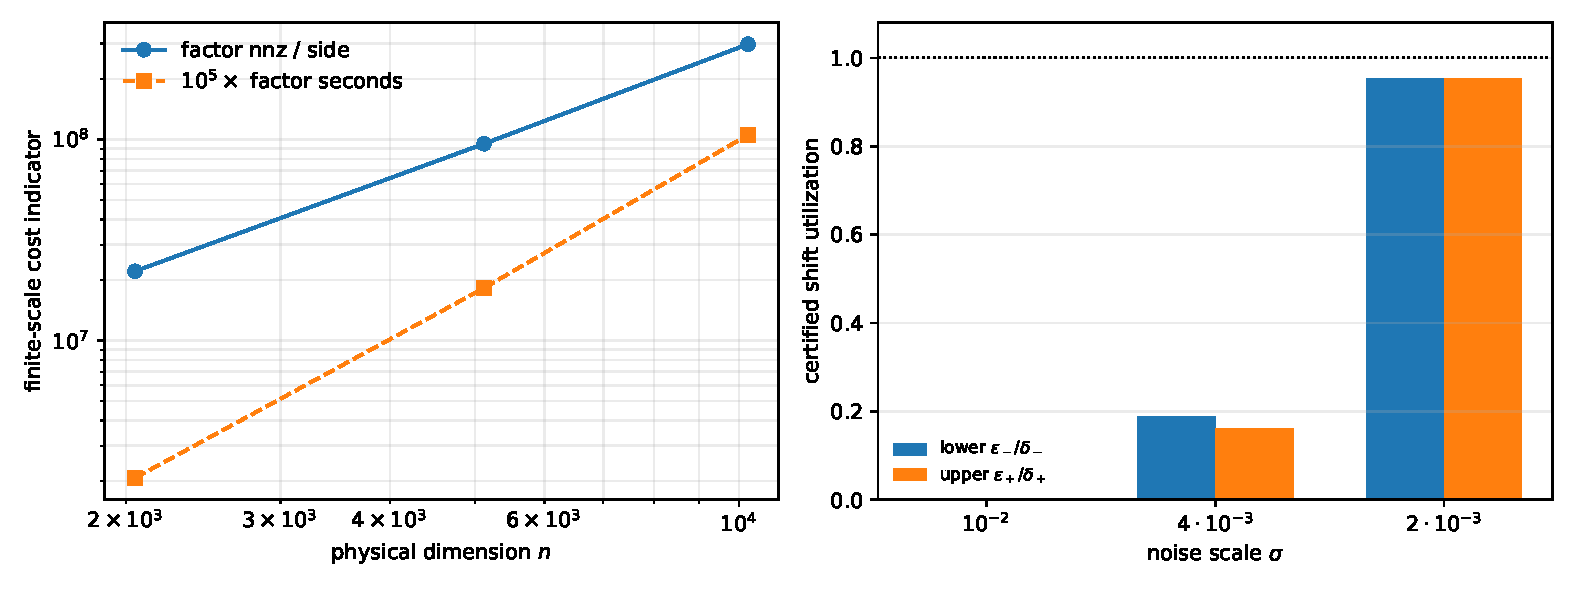
\includegraphics[width=0.98\textwidth]{figures/threshold_inertia_scaling.pdf}
\caption{Finite-scale diagnostics.  Left: factor nonzeros and one-side wall
time after a visual rescaling.  Right: the rigorous utilization
$\varepsilon_\pm/\delta_\pm$; the dotted line is the admissibility boundary.
The third scale is close but remains strictly below one.}
\label{fig:scaling}
\end{figure}

\subsection{Why asymmetric shifts matter}

At $\sigma=4\times10^{-3}$ and threshold factor two, the symmetric choice
$\delta=5.0\times10^{-4}$ gave correct pivot counts on both sides, but the
upper error grew to $1.1293\times10^{-3}$ and failed.  Moving symmetrically
to $\delta=5.6\times10^{-4}$ reduced the upper error to
$1.0457\times10^{-4}$ under the original $32N$ audit, but increased the
lower error to $7.0058\times10^{-4}$.  The selected asymmetric pair keeps
the stable lower factor from the first run and the stable upper factor from
the second.  This is an actual gain in theorem design, not merely a tuning
convenience.


\section{Complexity, negative findings, and scope}
\label{sec:scope}

\subsection{Fixed-factor architecture}

The certificate requires exactly two selected sparse factorizations and
linear postprocessing in their stored nonzeros.  It replaces the $n$ physical
right-hand sides of RH-30 by pivot signs and normwise backward errors.
This does not imply linear or near-linear asymptotic complexity: fill remains
the controlling quantity.  Fits over only three finite data points give
\begin{equation}
 \operatorname{nnz}(L+U)\sim n^{1.61},\qquad
 t_{\rm factor}\sim n^{2.44},\qquad
 M_{\rm peak}\sim n^{1.51}.
 \label{eq:empirical-exponents}
\end{equation}
These are descriptive fits, not asymptotic theorems.  The practical gain is
that the third scale closes with two factors and $O(\operatorname{nnz})$
verification; the method is not automatically cheaper at small scales.

\subsection{Discarded routes}

Three negative findings delimit the successful corridor.
\begin{enumerate}
 \item A cancellation-free scalar comparison solve for
       $\|U^{-1}L^{-1}\|_2$ produced a coarse candidate of order
       $2.12\times10^{65}$ and is useless here.
 \item Direct elimination of the untransformed shifted dilation starts from
       the small diagonal $-\alpha$ and suffers tiny-pivot instability.  The
       pair Hadamard congruence repairs that structural defect.
 \item A common symmetric shift is unnecessarily restrictive.  Sparse pivot
       growth can occur on opposite sides at nearby distances, even though
       exact inertia is unchanged.
\end{enumerate}
These failures do not contradict the spectral target; they identify
certificate mechanisms that discard too much cancellation or impose the
wrong numerical geometry.

\subsection{What is and is not proved}

The exact theorem concerns three finite stored matrices.  Combined with the
preceding one-channel reduction, it closes three selected lifted-resolvent
gates.  It does \emph{not} by itself:
\begin{enumerate}
 \item certify every arc of the archived contour;
 \item prove a contour root count;
 \item pass to zero noise or a continuum operator;
 \item construct a self-adjoint Hilbert--P\'olya operator;
 \item identify any eigenvalue with a nontrivial zeta zero;
 \item imply the Riemann hypothesis.
\end{enumerate}


\section{Outlook}
\label{sec:outlook}

The next technical problem is no longer conceptual.  The threshold-inertia
route is exact, but the third-scale utilization is about $0.954$.  Further
progress can come from:
\begin{enumerate}
 \item pair-level nested dissection or problem-specific separators to reduce
       threshold fill;
 \item a sharper verified bound for $\||L||U|\|_F$ that retains block
       orthogonality instead of summing all outer-product norms;
 \item verified multifrontal $LDL^*$ with symmetric pivot blocks, avoiding
       the $LU$-to-$LDL^*$ conversion term;
 \item independent asymmetric shift selection at each finer scale;
 \item reuse or updating of symbolic factors across nearby shifts.
\end{enumerate}
Any such extension should preserve the present architecture: exact target
enclosure, explicit rounding assumptions, a Hermitian inertia center, and a
Weyl sandwich whose final inequalities can be independently audited.


\section*{Reproducibility}

The repository directory
\begin{center}
\url{https://github.com/maris205/prime_dynamics_theory/tree/main/papers/RH-31-sparse-threshold-inertia}
\end{center}
contains the source, tests, factorization drivers, original failed pilots,
derived operation-count archives with SHA-256 provenance, summary tables,
and figure scripts.  The principal certificate files are
\begin{itemize}
 \item \texttt{results/exact\_target\_inertia\_sigma\_1e-2\_op24.json},
 \item \texttt{results/exact\_target\_inertia\_sigma\_4e-3\_op24.json},
 \item \texttt{results/exact\_target\_inertia\_sigma\_2e-3.json}.
\end{itemize}
The tests include dense singular-threshold equivalence, exact pair
congruence, asymmetric inertia recovery, exact channel Schur algebra,
bit-reversible power-of-two balancing, and a 100-digit enclosure cross-check.

\section*{Acknowledgments}

The numerical experiments were performed with NumPy, SciPy/SuperLU,
python-flint/Arb, mpmath, and Matplotlib.  The author thanks the developers of
these open-source packages.

\bibliographystyle{plainnat}
\bibliography{references}

\end{document}
